\documentclass[a4paper, 12pt]{article}
\input{general/preamble}

% Global table formatting consistency
\captionsetup[table]{skip=8pt}
\renewcommand{\arraystretch}{1.15}
\setlength{\extrarowheight}{1pt}
\setlength{\LTpre}{8pt}
\setlength{\LTpost}{8pt}

% Risk matrix colours
\definecolor{riskL}{RGB}{56, 142, 60}
\definecolor{riskM}{RGB}{74, 68, 0}
\definecolor{riskH}{RGB}{229, 83, 80}
\definecolor{riskDark}{RGB}{33, 33, 33}
\definecolor{riskGray}{RGB}{238, 238, 238}

\begin{document}

% Front cover (PDF)
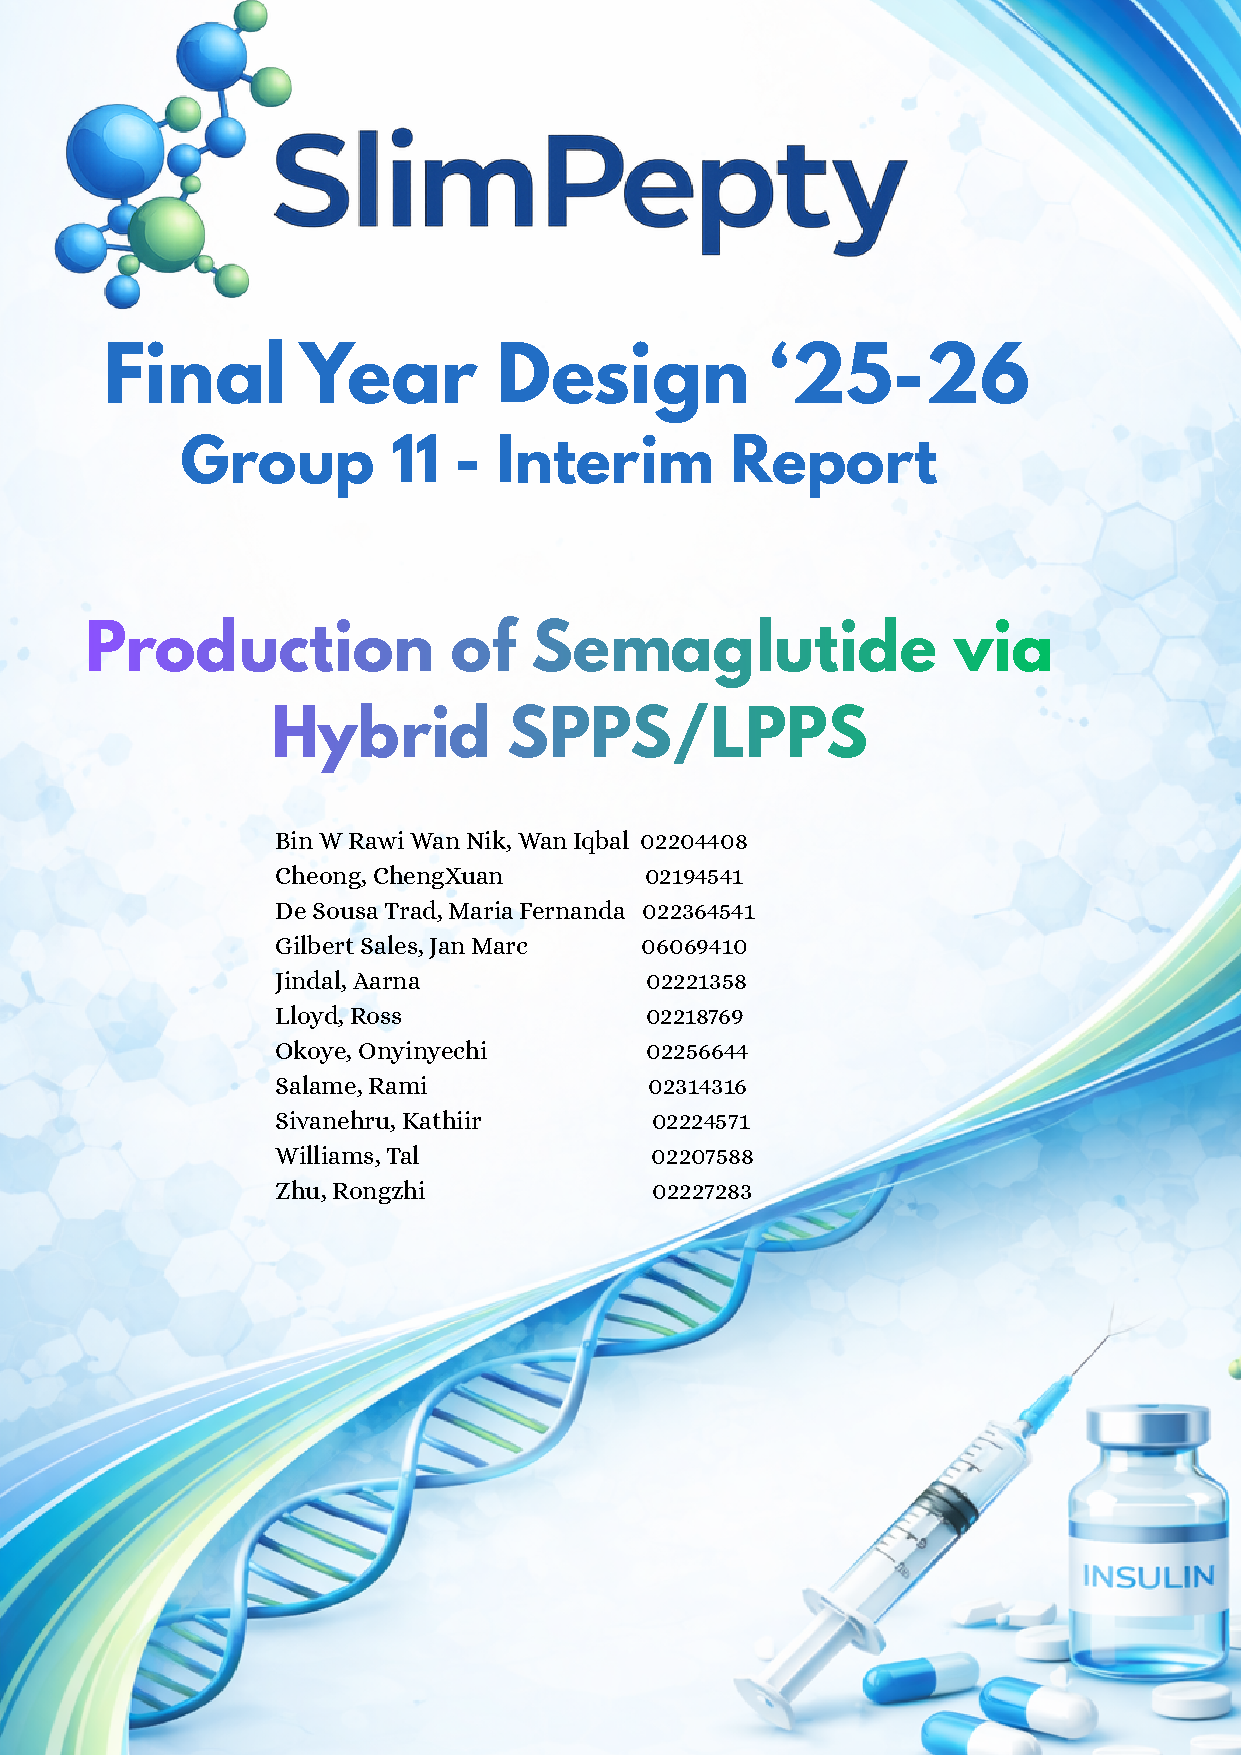
\includepdf[pages={1}]{figures/figure/interim_front_cover.pdf}

\tableofcontents
\newpage

\section*{Abbreviations}
\addcontentsline{toc}{section}{Abbreviations}

\begin{longtable}{@{}lp{0.75\textwidth}@{}}
\textbf{Abbreviation} & \textbf{Full Form} \\[4pt]
\endhead
API     & Active Pharmaceutical Ingredient \\
BAT     & Best Available Techniques \\
CCS     & Contamination Control Strategy \\
CDER    & Center for Drug Evaluation and Research \\
CDRH    & Center for Devices and Radiological Health \\
CEI     & Chemical Exposure Index \\
cGMP    & Current Good Manufacturing Practice \\
CIP     & Cleaning-In-Place \\
CMC     & Chemistry, Manufacturing and Controls \\
CSB     & Chemical Safety and Hazard Investigation Board \\
DCM     & Dichloromethane \\
DMF     & Dimethylformamide \\
FDA     & Food and Drug Administration \\
Fmoc    & 9-Fluorenylmethyloxycarbonyl \\
GLP-1   & Glucagon-Like Peptide-1 \\
GMP     & Good Manufacturing Practice \\
HAZOP   & Hazard and Operability Study \\
IED     & Industrial Emissions Directive \\
IND     & Investigational New Drug \\
ISD     & Inherently Safer Design \\
LPPS    & Liquid-Phase Peptide Synthesis \\
MIC     & Methyl Isocyanate \\
NBP     & N-Butylpyrrolidinone \\
NCL     & Native Chemical Ligation \\
NDA     & New Drug Application \\
NDEA    & N-Nitrosodiethylamine \\
NDMA    & N-Nitrosodimethylamine \\
OCP     & Office of Combination Products \\
OSCS    & Oversulfated Chondroitin Sulfate \\
PEL     & Permissible Exposure Limit \\
PIC/S   & Pharmaceutical Inspection Co-operation Scheme \\
PMI     & Process Mass Intensity \\
PMOA    & Primary Mode of Action \\
PSM     & Process Safety Management \\
RABS    & Restricted Access Barrier Systems \\
REACH   & Registration, Evaluation, Authorisation and Restriction of Chemicals \\
RP-HPLC & Reverse-Phase High-Performance Liquid Chromatography \\
SPPS    & Solid-Phase Peptide Synthesis \\
SVHC    & Substance of Very High Concern \\
TFA     & Trifluoroacetic Acid \\
TFF     & Tangential Flow Filtration \\
TWA     & Time-Weighted Average \\
VOC     & Volatile Organic Compound \\
WHO     & World Health Organization \\
ZLD     & Zero Liquid Discharge \\
\end{longtable}


\section{Introduction}

The design of a pharmaceutical manufacturing facility must ensure not only technical and economic feasibility but also the highest standards of safety, product quality, and environmental protection. This report evaluates the safety and environmental considerations associated with the proposed industrial production of semaglutide, a glucagon-like peptide-1 (GLP-1) receptor agonist widely used for the treatment of type-2 diabetes and obesity.

Semaglutide is a complex peptide manufactured through multi-step chemical synthesis and purification processes involving organic solvents and reactive reagents. As a result, the facility must operate under strict pharmaceutical quality standards while managing chemical hazards, occupational exposures, and waste streams generated during production. Failures in safety management or environmental protection within pharmaceutical manufacturing have historically led to severe consequences for patients, workers, and surrounding communities. Therefore, understanding lessons from past industrial incidents and integrating them into plant design is essential for preventing similar failures.

This report applies the principles of Best Available Techniques (BAT) \cite{EU_IED_2010_75} and inherently safer design (ISD) \cite{Yang_ISD_2018} to minimise hazards at the source rather than relying solely on downstream controls. BAT involves adopting the most effective and advanced methods that are technically and economically viable to reduce environmental impact, emissions, and waste generation. Inherently safer design principles (minimisation, substitution, moderation, and simplification) are incorporated where possible to reduce the quantity of hazardous materials handled, replace hazardous substances with safer alternatives, and simplify process operations to limit the potential for accidents.

Moreover, applicable safety and environmental legislation governing pharmaceutical production are reviewed. Based on this context, structured risk assessment methods such as qualitative risk assessment and Hazard and Operability Study (HAZOP) are used to identify potential process hazards and inform appropriate safeguards, mechanical integrity considerations, and site layout decisions. The environmental impact of the plant is also assessed through evaluation of raw material selection, waste disposal routes, as well as utilities and greenhouse gas emissions. Overall, this section informs the development of safe operating practices and effective waste management strategies to ensure the facility operates safely, sustainably, and in compliance with modern pharmaceutical manufacturing standards.


\clearpage
\section{Safety Considerations}

The safety of the proposed semaglutide manufacturing process is evaluated by considering both occupational exposure risks and product quality requirements. Tolerable exposure limits for the key chemicals used within the process were identified and compared with established occupational safety guidelines. These values inform the handling, containment, and ventilation requirements within the plant. This section also examines how safety considerations influence the overall plant layout, including equipment spacing, segregation of hazardous operations, and safe material handling routes. These design decisions aim to minimise risks to personnel, prevent cross-contamination, and ensure safe operation throughout the facility.

Product safety is also governed by strict pharmaceutical quality standards. Although the exact purity specification for semaglutide is not publicly disclosed in regulatory documents, literature and patent sources consistently indicate a target purity of approximately 99\%, which aligns with typical regulatory expectations for injectable pharmaceutical products \cite{Ashraf_semaglutide_2024, EP4181946A1_semaglutide_purification}. Compliance with the quality and safety standards established by the U.S. Food and Drug Administration (FDA), including the approval of semaglutide developed by Novo Nordisk, provides the regulatory benchmark that the proposed process must satisfy \cite{FDA_DrugsAtFDA, FDA_semaglutide_ChemR_2019}.

\subsection{Review of Historical Incidents}

\subsubsection{Quality Assurance Incidents}

In 1937, the S.E. Massengill Company (USA) formulated a new drug called ``Elixir Sulfanilamide'' by dissolving the widely used antibacterial drug sulfanilamide in diethylene glycol, an antifreeze chemical that is highly toxic to humans. No toxicity tests were performed, despite literature indicating its danger, which was a fundamental root cause of the disaster. The firm's control laboratory checked the product only for flavour, appearance, and fragrance, then shipped 633 lots across the country, leading to more than 100 deaths \cite{FDA_Sulfanilamide}. Many children who were prescribed this drug for sore throats developed severe abdominal pain, vomiting, anuria, convulsions, and ultimately died from kidney failure over 2--22 days \cite{Wax_1995}. Once physicians identified diethylene glycol as the toxic agent, the company issued vague recall telegrams, but under pressure from the FDA, a stronger recall followed. The tragedy exposed gaps in the Pure Food and Drug Act of 1906, which did not require drug safety testing, and led to the passage of the Federal Food, Drug, and Cosmetic Act of 1938. This law established mandatory pre-market safety evaluation and contributed to the foundations of modern Good Manufacturing Practice (GMP) \cite{FDA_Sulfanilamide, Wax_1995}.

Another major incident was the 2008 heparin contamination crisis. In early 2008, clinicians and regulators in the United States observed a sharp increase in severe allergic-type reactions and hypotension during administration of Heparin. Investigations traced these events to certain lots of intravenous heparin whose active ingredient, sourced from China, had been deliberately adulterated with oversulfated chondroitin sulfate (OSCS) \cite{Liu_2009, Kishimoto_2008}. OSCS is a highly sulfated glycosaminoglycan that closely resembled heparin in traditional pharmacopeial tests but is biologically distinct. The root causes of the crisis included heavy reliance on a globalised, cost-driven supply chain with limited oversight of upstream crude heparin processing workshops, as well as outdated pharmacopeial assays that lacked sufficient specificity to distinguish OSCS from authentic heparin \cite{Liu_2009}. These technical failures were compounded by broader systemic weaknesses discussed in the quality and reproducibility literature, including inadequate analytical validation, insufficient incentives to rigorously verify critical materials, and fragmented regulatory authority across international borders, which collectively allowed the adulteration to evade detection \cite{Liu_2009, Szajek_2016}. Once the pattern of adverse reactions was recognised, U.S. and international authorities rapidly coordinated targeted analytical testing, traced complex distribution chains, and implemented large-scale recalls of suspect heparin lots. The incident resulted in hundreds of serious adverse events and dozens of deaths, while disrupting global heparin supply for surgeries and dialysis \cite{Liu_2009, Kishimoto_2008}. In response, regulators strengthened pharmacopeial standards, introduced orthogonal analytical testing for routine lot release, and increased oversight of foreign active pharmaceutical ingredient manufacturers. The crisis highlighted the vulnerability of biologically derived medicines to sophisticated adulteration and prompted broader reforms to improve traceability, analytical robustness, and quality assurance across global pharmaceutical supply chains \cite{Liu_2009, Szajek_2016}.

The 2018 sartan (valsartan) nitrosamine crisis emerged when regulators detected nitrosamine impurities ($N$-Nitrosodimethylamine or NDMA and $N$-Nitrosodiethylamine or NDEA) in certain batches of the antihypertensive drug Valsartan and related angiotensin-II receptor blockers (``sartans''). These impurities are classified as probable human carcinogens, and their detection above acceptable limits led to widespread product recalls across Europe and other regions \cite{Wichitnithad_2023, EMA_Nitrosamine}. Investigations linked the contamination to changes in API manufacturing processes, particularly during synthesis of the tetrazole ring present in sartans. The use of nitrosating agents such as sodium nitrite together with amines or contaminated solvents created conditions that allowed unintended nitrosamine formation, a risk that earlier routine quality assays had not detected \cite{Wichitnithad_2023, Lowe_Sartan}. Regulators, including the European Medicines Agency, responded by recalling affected products, requiring manufacturers to review and modify synthesis processes, and introducing temporary limits for nitrosamine impurities while improved testing methods were developed \cite{EMA_Nitrosamine}. The crisis led to withdrawal of multiple sartan medicines and prompted a broader reassessment of impurity control in chemically synthesised drugs. In the aftermath, regulators strengthened guidance on nitrosamine risk assessment, harmonised analytical testing standards, and reinforced global quality assurance frameworks to improve detection and prevention of unexpected contaminants in pharmaceutical manufacturing \cite{EMA_Nitrosamine, Lowe_Sartan}.

\subsubsection{Worker Safety Incidents}

On 3 December 1984, at the Union Carbide India Limited pesticide plant in Bhopal, Madhya Pradesh, a catastrophic leak of methyl isocyanate (MIC) gas and other toxic chemicals occurred when large quantities of MIC were unintentionally released from storage tanks, creating a dense cloud that drifted over nearby residential areas and exposed hundreds of thousands of workers and local residents to lethal toxic gas \cite{Broughton_2005, Britannica_Bhopal}. The root causes included severe safety lapses and chronic underinvestment in hazard controls: critical safety systems such as refrigeration, vent scrubbers, and alarms were poorly maintained or non-functional, multiple backup safeguards were absent or disabled to cut costs, and safety training and staffing were profoundly inadequate, leaving workers unable to recognise or respond effectively to a runaway reaction and rising tank pressures \cite{Broughton_2005}. The disaster overwhelmed local health services, caused mass casualties with thousands killed within hours, and provoked urgent emergency involvement by authorities and medical personnel to treat respiratory distress and other acute toxic effects in exposed populations \cite{Britannica_Bhopal}. A large number of survivors suffered chronic respiratory, neurological, and other health problems, while families, communities, and workers faced long-lasting social and economic disruption \cite{Broughton_2005}. The Indian government then enacted landmark legislation such as the Environment (Protection) Act of 1986 to strengthen regulation of hazardous industries and mandated new public liability and compensation frameworks and legal actions were pursued against Union Carbide. This disaster has been a stark lesson in the consequences of poor industrial safety culture and the need for rigorous worker protection standards worldwide \cite{Broughton_2005, Britannica_Bhopal}.

On January 29, 2003, a catastrophic dust explosion and fire occurred at the West Pharmaceutical Services rubber manufacturing plant in Kinston, North Carolina, when a large accumulation of polyethylene dust generated during routine rubber processing and built up unnoticed above a suspended ceiling. This was ignited, resulting in a powerful blast that killed six workers and injured 38 others, including two firefighters, and destroyed much of the facility \cite{Blair_2007, CSB_West}. The root causes of the disaster were traced to critical management and engineering failures: West had not conducted adequate hazard assessments for the use of combustible powders, failed to consult or implement relevant industrial fire safety standards, did not effectively review material safety data sheets to recognise combustible dust hazards, and lacked a hazard communication programme that made workers aware of these risks \cite{Blair_2007}. Emergency crews evacuated and treated injured personnel, fire suppression efforts continued for days, and the U.S. Chemical Safety and Hazard Investigation Board (CSB) launched an in-depth investigation that highlighted the need for improved dust control and regulatory oversight \cite{Blair_2007, CSB_West}. In addition to the tragic loss of life and injuries, the explosion shattered the plant infrastructure, led to the loss of jobs, and underscored the hidden dangers of poorly managed combustible dust in the workplace \cite{Blair_2007}. In the aftermath, the CSB issued substantive safety recommendations emphasizing the need for engineering controls to prevent dust accumulation, adoption of NFPA combustible dust standards at the facility and statewide, improved hazard communication and worker training, and enhanced fire code enforcement; these administrative actions aimed to reduce the likelihood of similar incidents and to strengthen worker protection and industrial safety practices across industries handling combustible powders \cite{Blair_2007, CSB_West}.

In 2001, a significant worker radiation overexposure incident occurred at a licensed radiopharmaceutical manufacturing facility operated by Bristol-Myers Squibb Radiopharmaceuticals, Inc. (USA), when two workers received extremity doses far exceeding regulatory limits during routine preparation of radiopharmaceutical doses \cite{NRC_EA02160}. The root causes of the exposure were linked to inadequate control and assessment of radiation fields during hands-on preparation tasks, including insufficient use of appropriate shielding and failure to perform task-specific dose assessments that accounted for high exposure areas such as the fingertips, rather than relying solely on general dosimetry \cite{NRC_EA02160}. The licensee was cited with a Severity Level II violation, required to undertake corrective measures such as revising procedures, enhancing shielding and monitoring practices, and improving worker training on radiation hazards to prevent recurrence \cite{NRC_EA02160}. This heightened awareness of extremity dose risks among workers and regulators, prompting on-site reviews of similar operations at other facilities, while the after-effects encompassed strengthened radiation protection practices within the organization and greater emphasis by NRC on ensuring that licensees use dosimetry and controls appropriate to the magnitude and nature of tasks being performed \cite{NRC_EA02160}.

\subsubsection{Toxic Waste Disposal Incidents}

The Love Canal incident in Niagara Falls, New York, shows the dangers posed by improper hazardous waste disposal when industrial practices, urban development, and lack of environmental oversight converge. Originally dug as a canal, the site became a municipal and industrial chemical dumpsite from the 1940s through the early 1950s, with over 20,000 tons of toxic wastes buried there by Hooker Chemical Company, including carcinogens and other hazardous compounds \cite{EPA_LoveCanal, LevinCenter_LoveCanal}. In 1953 the company sold the property to the local school board, and homes, parks, and an elementary school were later built atop the landfill without adequate containment measures or long-term monitoring, leaving buried waste vulnerable to migration \cite{LevinCenter_LoveCanal, Geneseo_LoveCanal}. By the late 1970s, residents began reporting chemical residues in backyards, basements, and playgrounds, and state officials detected toxic chemicals leaching into the soil and groundwater, leading to serious health concerns including elevated incidences of miscarriages, birth defects, cancers, and respiratory problems in the community; hundreds of families ultimately required evacuation \cite{EPA_LoveCanal, LevinCenter_LoveCanal}. Emergency actions by authorities and investigations by the United States Environmental Protection Agency led to long-term remediation efforts such as landfill capping, leachate treatment, and site monitoring. The disaster ultimately prompted the creation of the Comprehensive Environmental Response, Compensation, and Liability Act (Superfund) in 1980, establishing a national framework for identifying and cleaning up hazardous waste sites \cite{LevinCenter_LoveCanal}. In the ensuing decades, this incident reminded regulators, workers, and communities of the critical importance of proper waste disposal, long-term oversight, and environmental health protections \cite{EPA_LoveCanal, LevinCenter_LoveCanal, Geneseo_LoveCanal}.

The Probo Koala Toxic Waste Dumping occurred in August 2006 when the cargo ship Probo Koala, chartered by Trafigura, illegally discharged large quantities of hazardous petroleum-processing waste around Abidjan, C\^{o}te d'Ivoire after failing to secure proper disposal in Europe \cite{Amnesty_Trafigura}. The waste was a caustic mixture of petroleum residues and chemical by-products and was spread at numerous open sites on the night of 19 August, releasing toxic fumes that sickened tens of thousands of people with symptoms such as headaches, skin and respiratory irritation, vomiting, and breathing difficulties, leading to at least 15 deaths and over 100,000 people seeking medical treatment \cite{BBC_Trafigura, Amnesty_Trafigura}. The disaster was driven by corporate cost-cutting, inadequate risk assessment, and exploitation of weak regulatory oversight in waste disposal regions \cite{Amnesty_Trafigura, DOJ_EOIR}. Emergency medical responses and clean-up operations were organised by local authorities and international agencies, while Trafigura later reached financial settlements with affected communities. The incident triggered international scrutiny of hazardous waste export practices, legal penalties for illegal waste export, and calls for stronger global enforcement of hazardous waste regulations \cite{Amnesty_Trafigura, DOJ_EOIR}.

The Hyderabad pharmaceutical pollution crisis (2000s--present, India) illustrates the environmental risks of inadequate waste management in pharmaceutical manufacturing. The city has faced persistent contamination from untreated or poorly treated wastewater containing antibiotics and other pharmaceutical residues released into rivers and groundwater \cite{Nordea_Hyderabad}. Studies have detected extremely high concentrations of drug residues in local water systems, creating conditions that promote the development of antibiotic-resistant bacteria (``superbugs'') and posing a growing global public health concern \cite{TBIJ_Superbugs}. The root causes include inadequate wastewater treatment capacity at manufacturing facilities, lax enforcement of environmental standards, and the absence of robust pollution controls within pharmaceutical regulatory frameworks, which have traditionally prioritised product quality over environmental protection \cite{Nordea_Hyderabad, TBIJ_Superbugs}. In response, state authorities have launched intensified enforcement actions against polluting bulk drug units, demanding adoption of improved waste management practices such as Zero Liquid Discharge (ZLD) systems, enhanced effluent monitoring, and penalties for non-compliance to curtail dangerous discharges \cite{NIE_Telangana}. Additionally, on 23 January 2020 the Ministry of Environment, Forest and Climate Change introduced the world's first regulatory standards limiting antibiotic concentrations in pharmaceutical wastewater, aiming to reduce environmental drivers of antimicrobial resistance \cite{ReActGroup_India}.

\subsubsection{Transferable Lessons}

Across these incidents, several critical lessons emerge for pharmaceutical manufacturing. These events collectively demonstrate the necessity of rigorous pre-market safety testing, verification of raw materials and intermediates, and strict control of manufacturing process changes to prevent unexpected impurities or adulteration. They also highlight the importance of comprehensive hazard identification and risk assessment (e.g., chemical toxicity, combustible dust, radiation exposure), well-maintained safety systems, and thorough worker training to ensure safe plant operations. Furthermore, they underline the need for strong regulatory compliance and effective pharmacovigilance to rapidly detect and respond to safety issues. Environmental incidents reveal that responsible waste management, effective effluent treatment, and pollution controls are essential to prevent long-term ecological and public health damage. In designing this semaglutide manufacturing process, these lessons are incorporated through strict adherence to GMP, incorporating methods for impurity and contaminant monitoring, comprehensive process hazard analyses, engineered safety controls for hazardous materials and dust, and adequate waste treatment strategies. Together, these measures aim to ensure product quality, worker safety, regulatory compliance, and environmental protection throughout the lifecycle of the manufacturing process.

\subsection{Local Legislation: Safety}

\subsubsection{FDA Drug Approval}

Under Section 505 of the Federal Food, Drug, and Cosmetic Act (FD\&C Act), any drug product sold in the United States must be covered by an approved New Drug Application (NDA) \cite{eCFR_21CFR50}. Since semaglutide is already approved by the FDA in the form of Novo Nordisk's Ozempic (NDA 209637) and Wegovy (NDA 216084), the most appropriate approval route for this facility is the 505(b)(2) pathway, established by the Hatch-Waxman Amendments of 1984 \cite{Allucent_505b2}. This hybrid route permits the applicant to rely in part on existing published data or the FDA's prior findings of safety and effectiveness for a reference listed drug, supplemented by new studies conducted by the applicant, avoiding the need to repeat the full innovator clinical programme \cite{Salminen_2023}.

Two separate regulatory submissions are required: one for the drug substance (API) and one for the finished injectable drug product. Prior to NDA submission, an Investigational New Drug (IND) application must be filed if new clinical studies are needed, followed by Phase I, II, and III clinical trials. The Chemistry, Manufacturing and Controls (CMC) module of the NDA must comprehensively address the manufacturing process, analytical methods, specifications, container closure system, and stability data for both the API and the finished product \cite{Vici_505b}.

\subsubsection{Current Good Manufacturing Practice (cGMP)}

In addition to the product approval pathway, SlimPepty must operate in compliance with current Good Manufacturing Practice (cGMP) requirements for both the semaglutide drug substance and the finished injectable drug product. For the API, the principal GMP standard is ICH Q7, which sets out requirements for quality management, personnel, buildings and facilities, process equipment, documentation, production controls, laboratory controls, validation, and change management \cite{FDA_Q7}. For the finished injectable product, the applicable GMP framework is 21 CFR Parts 210 and 211, which govern the manufacture, processing, packing, and holding of drug products \cite{FDA_cGMP}. These regulations require written production and process control procedures, quality unit oversight, scientifically sound laboratory controls, and appropriate cleaning, maintenance, and documentation systems to ensure that each batch consistently meets its required identity, strength, quality, and purity \cite{eCFR_211}. For SlimPepty, this means that batch records, deviation investigations, cleaning validation, analytical release testing, and change control must be embedded into the site's pharmaceutical quality system across both the synthesis and fill-finish sections of the plant.

\subsubsection{Combination Product Regulations}

A pre-filled pen injector containing semaglutide solution constitutes a drug-device combination product as defined in 21 CFR 3.2(e), as it comprises both a drug and a device constituent combined into a single entity \cite{FDA_ComboGMP_2017}. The FDA's Office of Combination Products (OCP) designates regulatory lead to the centre whose jurisdiction corresponds to the product's Primary Mode of Action (PMOA). Since the therapeutic effect of semaglutide arises from its pharmacological action as a GLP-1 receptor agonist, the Center for Drug Evaluation and Research (CDER) leads the premarket review, with the Center for Devices and Radiological Health (CDRH) providing secondary oversight of the pen injector \cite{Latoz_2023}.

Manufacturing compliance for combination products is governed by 21 CFR Part 4, which requires the facility to satisfy the current good manufacturing practice (cGMP) requirements of both drug regulations (21 CFR Parts 210 and 211) and the device Quality Management System Regulation (21 CFR Part 820 and ISO 13485) \cite{eCFR_Part4}. This additionally requires the maintenance of a Design History File for the pen injector, human factors and usability testing, extractables and leachables assessment for all device-contact materials, and dose delivery accuracy testing to the ISO 11608 series for needle-based injection systems \cite{FDA_Aseptic_2004}.

\subsubsection{Sterile Injectable Manufacturing}

Producing a finished injectable drug product subjects the facility to the full scope of FDA sterile drug product cGMP requirements under 21 CFR Part 211 and the FDA Guidance for Industry: Sterile Drug Products Produced by Aseptic Processing (2004) \cite{eCFR_211_Sterile}. Since semaglutide is a thermolabile peptide that cannot be terminally sterilised, the finished product must be manufactured by aseptic processing, in which sterilised drug solution is filled into pre-sterilised containers under conditions that preclude microbial contamination. The facility must therefore incorporate dedicated cleanroom infrastructure, including ISO Class 5 (Grade A) conditions in the critical filling zone and ISO Class 7 (Grade B) in the surrounding background environment.

Additional requirements applicable specifically to injectable finished products under 21 CFR Part 211 include endotoxin and pyrogen control, 100\% visual inspection of all filled units for cracks and visible particulates, sterility testing per USP $\langle$71$\rangle$, container closure integrity testing throughout shelf life, and comprehensive product labelling including patient instructions for use. All aseptic processes must be validated through periodic aseptic process simulations (media fills).

\subsubsection{Sterile Manufacturing International Benchmark}

EU GMP Annex 1, Manufacture of Sterile Medicinal Products, was comprehensively revised in August 2022 and came into force on 25 August 2023, developed jointly by the European Commission, the Pharmaceutical Inspection Co-operation Scheme (PIC/S), and the World Health Organization (WHO) \cite{EC_Annex1_2022}. It constitutes the global benchmark for sterile pharmaceutical manufacturing and is binding for any product sold in EU or UK markets.

The 2022 revision introduced a mandatory site-wide Contamination Control Strategy (CCS): a documented framework connecting contamination risks, engineering controls, and monitoring across all areas of the facility. It also establishes that Restricted Access Barrier Systems (RABS) or isolators should be used to minimise human intervention in the critical filling zone, and that any contaminated unit in an aseptic process simulation constitutes a failed run, requiring full investigation and three consecutive passing runs before commercial manufacturing may resume \cite{HoganLovells_Annex1}.

\subsubsection{Process Safety Management}

The OSHA standard for Process Safety Management of Highly Hazardous Chemicals (PSM), codified at 29 CFR 1910.119, applies to any process holding flammable liquids with a flashpoint below 37.8\textdegree{}C in a quantity of 10,000~lbs (4,536~kg) or more at a single location \cite{OSHA_PSM}. Given the large volumes of low-flashpoint solvents required for peptide synthesis at 237~kg/year production scale, including acetonitrile (flashpoint 2\textdegree{}C) and dichloromethane (DCM), the facility is expected to fall under PSM coverage. PSM requires the facility to implement a comprehensive process safety programme encompassing Process Hazard Analysis (PHA), written operating procedures, mechanical integrity management, management of change (MOC) procedures, emergency planning, and compliance audits at a minimum every three years. North Carolina operates its own OSHA-approved State Plan (NC OSH Division) under 29 CFR 1902, which applies PSM requirements in substantively identical form to the federal rule.

\subsubsection{Hazard Communication and Occupational Exposure Limits}

The OSHA Hazard Communication Standard (HazCom 2012, 29 CFR 1910.1200), aligned with the Globally Harmonised System (GHS), requires that all hazardous chemicals in the workplace are properly classified, labelled, and accompanied by Safety Data Sheets (SDS), and that employees receive training on the chemicals they work with \cite{OSHA_HazCom}. OSHA establishes Permissible Exposure Limits (PELs) for workplace chemicals under 29 CFR 1910.1000, which are directly applicable to the solvents used in this process: dimethylformamide (DMF) is subject to a PEL of 10~ppm (8-hour time-weighted average (TWA)); acetonitrile 40~ppm; and DCM 25~ppm, the latter also requiring specific medical surveillance given its classification as a suspected human carcinogen. For piperidine and trifluoroacetic acid (TFA), for which no OSHA PELs have been established, the employer must ensure exposures remain safe under the general duty clause of the OSH Act (29 U.S.C. 654(a)(1)). Engineering controls, including local exhaust ventilation and enclosed handling systems, must serve as the primary means of exposure control, with personal protective equipment as a secondary measure.

\subsection{Qualitative Risk Assessment}

A qualitative risk assessment was conducted to identify major hazards associated with the process and assess the risks to personnel, equipment, and the environment. The multidisciplinary RA/HAZOP team is listed in Table~\ref{tab:ra_hazop_team}. Hazards were evaluated based on their likelihood of occurrence and the severity of potential consequences, and appropriate control measures were identified. The likelihood and severity classifications used, as well as the risk matrix applied, are provided in Appendix~XX (Tables~\ref{tab:likelihood}, \ref{tab:severity}, and~\ref{tab:riskmatrix}).

\subsection{Mechanical Integrity}

Table~\ref{tab:material_selection} summarises the materials selected for the different equipment across the plant, together with the justification for each choice. GMP considerations are incorporated into the design, with material selection accounting for both chemical compatibility with process streams and appropriate pharmaceutical manufacturing standards.

\setlength{\LTleft}{0pt}
\setlength{\LTright}{0pt}
\footnotesize
\begin{longtable}{|>{\raggedright\arraybackslash}p{0.10\textwidth}|>{\raggedright\arraybackslash}p{0.14\textwidth}|>{\raggedright\arraybackslash}p{0.20\textwidth}|>{\raggedright\arraybackslash}p{0.14\textwidth}|>{\raggedright\arraybackslash}p{0.24\textwidth}|}
    \caption{Material selection for major process equipment.}
    \label{tab:material_selection}                                                                                                                                                                                                                                                                                                                                                                                                                                                                                                                                                                                                                                                                                                                                                                                                                                                                                                                                                                                                                                                                                                                                                                                                                                                                                                                                                                                                                                                                                                                                                                                                                                                                                                                          \\
    \hline
    \textbf{Process section} & \textbf{Equipment}                                                                                                                                                             & \textbf{Associated Chemicals}                                                                                                                                                                                                                                                                                                                                                                                                                                                                                                                                                                                                                                                                                                                                                                             & \textbf{Material selected}                                                 & \textbf{Justification}                                                                                                                                                                                                                                                                                                                                                                                                                                                                                                                                                                                                                             \\
    \hline
    \endfirsthead
    \hline
    \textbf{Process section} & \textbf{Equipment}                                                                                                                                                             & \textbf{Associated Chemicals}                                                                                                                                                                                                                                                                                                                                                                                                                                                                                                                                                                                                                                                                                                                                                                             & \textbf{Material selected}                                                 & \textbf{Justification}                                                                                                                                                                                                                                                                                                                                                                                                                                                                                                                                                                                                                             \\
    \hline
    \endhead
    \hline
    \endfoot
    \hline
    \endlastfoot
    Batch                    & Raw material storage tanks (T-1 to T-18)                                                                                                                                       & Fmoc-Gln(Trt)-OH, Fmoc-Gly-OH, Fmoc-Glu(OtBu)-OH, Fmoc-Leu-OH, Fmoc-Tyr(tBu)-OH, Fmoc-Ser(tBu)-OH, Fmoc-Val-OH, Fmoc-Asp(OtBu)-OH, Fmoc-Thr(tBu)-OH, Fmoc-Phe-OH, Fmoc-Aib-OH, Fmoc-His(Trt)-OH, Fmoc-Ile-OH, Fmoc-Ala-OH, Fmoc-Lys(Alloc)-OH, Fmoc-Trp(Boc)-OH, Fmoc-Arg(Pbf)-OH, Fmoc-AEEA-OH, Fmoc-Cys(Trt)-OH                                                                                                                                                                                                                                                                                                                                                                                                                                                                                         & 316L stainless steel, refrigerated at -20 C                                & 316L stainless steel was selected for raw material storage tanks due to its excellent resistance to corrosion by organic reagents and its widespread use in GMP-compliant pharmaceutical processing equipment. The smooth surface also allows for easier cleaning procedures, which is very important in a pharmaceutical plant due to risks of cross-contamination. Cheaper steels like 304 stainless steel are not used as they would not meet the GMP criteria.                                                                                                                                                                                 \\
    \hline
                             & Solvent storage tanks, except TFA and HCl, associated mixers and Frag 1 and 2 storage surge tanks (T-19 to T-23, T-25, T-26, T-29 to T-34, T-36 to 42, M-1, M-3, M-6, and M-7) & DMF, Piperidine, TBTU, DIEA, DCM, TIPS, H2O, AEEA, C-18, Pd, PhSiH3, NaNO2, Et2O, MESNa, Gn.HCl, Na2HPO4, Unusable peptides (frag 1), Peptide-S-C6H4-COOH (Fragment 1 MENSa Thioester), H-Cys-Ala-Lys(SideChain)-...-Gly-OH, Unusable peptides (frag 2)                                                                                                                                                                                                                                                                                                                                                                                                                                                                                                                                                   & 316L stainless steel                                                       & The compatibility chart for 316L stainless steel indicates good to excellent resistance to organic solvents, amines, and aqueous salt solutions, demonstrating that it is suitable for storing and processing these chemicals under typical operating conditions. Also, it allows for easier cleaning procedures.                                                                                                                                                                                                                                                                                                                                  \\
    \hline
                             & TFA and HCl storage and associated mixers (T-24, T-35, M-2, M-4, and M-6)                                                                                                      & TFA, TIPS, H2O, NaNO2, HCl, MESNa, H2O                                                                                                                                                                                                                                                                                                                                                                                                                                                                                                                                                                                                                                                                                                                                                                    & PTFE-lined 316L stainless steel                                            & PTFE shows excellent compatibility with HCl, which is more corrosive than TFA, implying that PTFE provides excellent resistance against strong mineral and organic acids.                                                                                                                                                                                                                                                                                                                                                                                                                                                                          \\
    \hline
                             & Resin storage (T-27 and T-28)                                                                                                                                                  & Fmoc-Hydrazine-2-CTC Resin, Resin-OH                                                                                                                                                                                                                                                                                                                                                                                                                                                                                                                                                                                                                                                                                                                                                                      & Original packaging, refrigerate the resin not in use at 2-8 C              & SPPS resins are typically supplied in moisture-controlled packaging and can degrade if exposed to humidity or heat, and to avoid that, they are stored in their original packaging.                                                                                                                                                                                                                                                                                                                                                                                                                                                                \\
    \hline
                             & Reactors (R-1 to R-3)                                                                                                                                                          & Gln (x1), Fmoc-Gly-OH, Fmoc-Leu-OH, Fmoc-Glu(OtBu)-OH, Fmoc-Tyr(tBu)-OH, Fmoc-Ser(tBu)-OH, Fmoc-Val-OH, Fmoc-Asp(OtBu)-OH, Fmoc-Thr(tBu)-OH, Fmoc-Phe-OH, Fmoc-Aib-OH, Fmoc-His(Trt)-OH, DMF, piperidine, TBTU, DIEA, TFA, TIPS, H2O, Fmoc-Hydrazine-2-CTC Resin, Spent Resin beads (SPPS1), Unusable peptides (frag 1), H-His(Trt)-...-Gln(Trt)-NHNH2 (Peptide Hydrazide), Ph3CH, tBuOH, (iPr)3Si-OOCCF3, C19H21N, C6H5N3O, C5H12N2O, DIEA*HBF4 (salt), DCM, Fmoc-AEEA-OH, Resin-OH, Fmoc-Ile-OH, Fmoc-Ala-OH, Fmoc-Lys(Alloc)-OH, Fmoc-Trp(Boc)-OH, Fmoc-Arg(Pbf)-OH, Fmoc-Cys(trt)-OH, H-Cys-Ala-Lys(SideChain)-...-Gly-OH, Unusable peptides (frag 2), Pd(PPh3)4 (Catalyst), PhSiH3, Spent resin beads (SPPS2), DIEAHCL, C9H12Si, NaNO2, HCl, MESNa, Peptide-S-C6H4-COOH (Fragment 1 MENSa Thioester) & Glass-lined 316L stainless steel                                           & Glass-lined steel reactors were selected for the peptide synthesis steps due to their excellent resistance to corrosion and chemical attack from aggressive reagents and solvents used in the process. The glass lining forms an inert, non-porous barrier that protects the underlying steel structure from acids, solvents, and other reactive chemicals, significantly extending equipment lifetime and preventing corrosion of the vessel. They are usually used when the product purity can not be compromised, and they meet GMP regulations. They also facilitate cleaning between batches, which as mentioned earlier is really important. \\
    \hline
                             & Separation units (S-1 to S-7)                                                                                                                                                  & DMF, TFA, TIPS, H2O, Spent resin beads (SPPS1), Spent resin beads (SPPS2), Unusable peptides (frag 1), Unusable peptides (frag 2), H-His(Trt)-...-Gln(Trt)-NHNH2 (Peptide Hydrazide), Ph3CH, tBuOH, (iPr)3Si-OOCCF3, Et2O, NaNO2, HCl, MESNa, Peptide-S-C6H4-COOH (Fragment 1 MENSa Thioester), H-Cys-Ala-Lys(SideChain)-...-Gly-OH                                                                                                                                                                                                                                                                                                                                                                                                                                                                       & Glass-lined 316L stainless steel                                           & Although PTFE-lined steel is usually cheaper than glass-lined steel and could have been used for this section as well, the economic compromise was justified by the more suitable properties of glass-lined steel.                                                                                                                                                                                                                                                                                                                                                                                                                                 \\
    \hline
    Continu-\newline ous     & MPAA storage vessel                                                                                                                                                            & MPAA                                                                                                                                                                                                                                                                                                                                                                                                                                                                                                                                                                                                                                                                                                                                                                                                      & 316L stainless steel, but refrigerate at 2-8 C and have a nitrogen blanket & According to the safety data sheet for MPAA, it needs to be stored under cold and dry conditions, with the container being tightly closed and under an inert gas (like nitrogen) because MPAA is combustible. It is an organic acid and should be compatible with 316L stainless steel.                                                                                                                                                                                                                                                                                                                                                            \\
    \hline
                             & Solvent storage tanks (T-43 to T-47), associated mixers (M-8 to M-10), reactors (R-4 and R-5), T-48 surge tank, and separators (S-8 to S-11)                                   & MPAA, TCEP, VA-044, GSH, acetonitrile, H2O, Frag 1, Frag 2, Frag 1 unusable, Frag 2 Unusable, Gn.HCl, H2O, Na2HPO4, MESNa, Frag 1 MPAA, Cys - Semaglutide, Semaglutide, TECP=O, GSSH, H2S                                                                                                                                                                                                                                                                                                                                                                                                                                                                                                                                                                                                                 & 316L stainless steel                                                       & This section of the plant does not contain any strong acids or bases which means that 316L stainless steel is a good choice for these equipment. It facilitates cleaning.                                                                                                                                                                                                                                                                                                                                                                                                                                                                          \\
    \hline
    Solvent recovery         & All equipment for this section (T-49, S-12 to S-14)                                                                                                                            & Fmoc-Gln(Trt)-OH, Fmoc-Gly-OH, Fmoc-Glu(OtBu)-OH, Fmoc-Leu-OH, Fmoc-Tyr(tBu)-OH, Fmoc-Ser(tBu)-OH, Fmoc-Val-OH, Fmoc-Asp(OtBu)-OH, Fmoc-Thr(tBu)-OH, Fmoc-Phe-OH, Fmoc-Aib-OH, Fmoc-His(Trt)-OH, Fmoc-Ile-OH, Fmoc-Ala-OH, Fmoc-Lys(Alloc)-OH, Fmoc-Trp(Boc)-OH, Fmoc-Arg(Pbf)-OH, Fmoc-Cys(trt)-OH, DMF, Piperidine, TBTU, DIEA, C19H21N, C6H5N3O, C5H12N2O, DIEA*HBF4 (salt), DIEA*HCl                                                                                                                                                                                                                                                                                                                                                                                                                  & 316L stainless steel                                                       & As mentioned above, all of the chemicals involved in this section have been found to be compatible with 316L stainless steel.                                                                                                                                                                                                                                                                                                                                                                                                                                                                                                                      \\
\end{longtable}
\normalsize

\subsection{HAZOP Summary}

A hazard and operability (HAZOP) analysis was conducted for the chosen subsection of the PFD, details of which are shown below: (node, design and op conditions)

\begin{table}[htbp]
    \centering
    \caption{RA and HAZOP study team members and assigned subteams.}
    \label{tab:ra_hazop_team}
    \small
    \begin{tabularx}{\textwidth}{|>{\raggedright\arraybackslash}X|>{\raggedright\arraybackslash}X|c|c|}
        \hline
        \textbf{Member}               & \textbf{Team}            & \textbf{Signature} & \textbf{Subteam} \\
        \hline
        Jindal, Aarna                 & Safety and Environmental & AJ                 & 1                \\
        \hline
        Gibert Sales, Jan Marc        & Safety and Environmental & JGS                & 2                \\
        \hline
        Lloyd, Ross                   & Synthesis                & RL                 & 1                \\
        \hline
        De Sousa Trad, Maria Fernanda & Reactor Design           & MFT                & 2                \\
        \hline
        Zhu, Alice                    & Separations              & AZ                 & 2                \\
        \hline
        Sivanehru, Kathiir            & Process Control          & KS                 & 1                \\
        \hline
        Williams, Tal                 & Synthesis                & TW                 & 2                \\
        \hline
        Salame, Rami                  & Process Control          & RS                 & 2                \\
        \hline
        Okoye, Onyi                   & Economics                & OO                 & 1                \\
        \hline
        bin W Rawi Wan Nik, Iqbal     & Separations              & WI                 & 1                \\
        \hline
        Cheong, Chenxuan              & Reactor Design           & CC                 & 1                \\
        \hline
    \end{tabularx}
    \normalsize
\end{table}

\begin{table}[htbp]
    \centering
    \caption{HAZOP node definition for the NCL--TFF--desulfuriser review.}
    \label{tab:hazop_node_definition}
    \small
    \begin{tabularx}{\textwidth}{|>{\raggedright\arraybackslash}p{0.2\textwidth}|>{\raggedright\arraybackslash}X|}
        \hline
        \textbf{Field} & \textbf{Details}                                                                                                                                                                                                                                                                                                                                                                \\
        \hline
        Node           & 1                                                                                                                                                                                                                                                                                                                                                                               \\
        \hline
        Project        & Semaglutide Production - NCL and Desulfuriser Review                                                                                                                                                                                                                                                                                                                            \\
        \hline
        Date           & 5-Mar-26                                                                                                                                                                                                                                                                                                                                                                        \\
        \hline
        Title          & Native chemical ligation or NCL reactor (R-4) to tangential flow filtration or TFF unit to desulfuriser reactor (R-5)                                                                                                                                                                                                                                                           \\
        \hline
        Objective      & The design intent of the NCL reactor is to join the 2 peptide fragments obtained from the upstream batch part of the process, whereas the TFF unit concentrates the peptides (as retentate) mainly by removing water. The concentrated stream is then sent to the desulfurisation reactor, where the ligation auxiliary group is removed to obtain the final peptide structure. \\
        \hline
        Node extent    & This node includes the flow streams from the surge tanks that store fragments 1 and 2, the NCL reactor, TFF unit, and desulfuriser reactor, including its outlet (F-95). The outlets of solvent storage tanks, pumps, and the utility lines within this part of the process are also considered.                                                                                \\
        \hline
    \end{tabularx}
    \normalsize
\end{table}

\begin{table}[htbp]
    \centering
    \caption{Design and operating conditions for the selected HAZOP node equipment.}
    \label{tab:hazop_design_operating_conditions}
    \footnotesize
    \begin{tabularx}{\textwidth}{|>{\raggedright\arraybackslash}p{0.2\textwidth}|>{\raggedright\arraybackslash}X|>{\raggedright\arraybackslash}X|>{\raggedright\arraybackslash}X|}
        \hline
        \textbf{}                     & \textbf{R-4 (NCL)} & \textbf{S-8 (TFF)} & \textbf{R-5 (Desulfuriser)} \\
        \hline
        \textbf{Design Conditions}    &
        Flow:\newline
        Pressure: 1.1 bar\newline
        Temperature: 328 K\newline
        Level:\newline
        pH: 5.9-8.3                   &
        Flow:\newline
        Pressure:\newline
        Temperature:                  &
        Flow:\newline
        Pressure: 5.5 bar\newline
        Temperature: 325 K\newline
        Level: 95\%                                                                                           \\
        \hline
        \textbf{Operating Conditions} &
        Flow:\newline
        Pressure: 1 bar\newline
        Temperature: 298 K\newline
        Level:\newline
        pH: 6.5-7.5                   &
        Flow:\newline
        Pressure:\newline
        Temperature:                  &
        Flow:\newline
        Pressure: 5 bar\newline
        Temperature: ?? K\newline
        Level: 95\%                                                                                           \\
        \hline
    \end{tabularx}
    \normalsize
\end{table}

The purpose of the study was to systematically identify potential process hazards and operability issues that could arise from deviations in key operating parameters such as flow, temperature, pressure, and pH within the node boundaries. The analysis assumed consistent operation outside the node boundaries, correct installation and design of equipment, steady state operation of the process equipment in the chosen node.

Key recommendations from this analysis are summarised in Table~XX. These measures aim to reduce the likelihood of process upsets while maintaining safe and reliable peptide processing within this section of the plant.

\subsection{Site Layout}

\subsubsection{Location}

SlimPepty's plant will be located in Research Triangle Park (RTP) near Raleigh, North Carolina, United States. RTP is a well-established biotechnology and pharmaceutical manufacturing hub hosting companies such as Novo Nordisk, Biogen, and Eli Lilly and Company. The park's low-density industrial zoning and large separation between facilities reduce potential off-site impacts in the event of accidental releases. Treated aqueous effluent from the plant can be discharged to the regional municipal sewer network, with final treatment at facilities such as the Neuse River Resource Recovery Facility.

\subsubsection{Layout of the Process}

The plant layout was developed using a risk-based approach, with the arrangement of process units and auxiliary facilities selected to reduce the consequences of fire, explosion, and toxic release while maintaining practical operation, maintenance, and emergency access \cite{Lees_2012}. Hazard assessment formed part of this layout development, and Dow's Chemical Exposure Index (CEI) was used in the siting of hazardous areas so that vulnerable or occupied spaces were kept away from zones of greater release consequence \cite{AIChE_CEI_1998}.

The main building contains the plant operation area together with the principal occupied rooms, while the higher-hazard external units are located away from the main occupied spaces. The control room is positioned beside the plant operation area so that operators can supervise the process closely without being located inside the production space. The quality check room is provided separately from the main production area, so it remains distinct from both the control room and the process floor itself.

Within the plant operation area, the equipment is arranged broadly according to a straight-line layout principle, following the sequence of manufacture from raw material and solvent/resin storage, through Fmoc handling and solid-phase peptide synthesis (SPPS) processing, then to activation and continuous processing. This gives a more logical production flow within the building and reduces unnecessary movement of materials between unit operations.

The Et$_2$O storage tank is located outside the main building and toward the northeast of the site because the main concern for diethyl ether is leakage leading to formation of a spreading liquid pool that evaporates rapidly, produces a flammable vapour cloud, and may ignite even before it is clearly visible. Locating the Et$_2$O tank externally reduces the likelihood that such a release would directly affect the main process building. The waste treatment plant is also located away from the principal occupied areas. Since the prevailing wind direction is from southwest to northeast, placing these units to the northeast of the main building helps reduce potential personnel exposure in the event of an accidental release.

Additional secondary containment was incorporated for hazardous liquid storage. The Et$_2$O tank is bunded on the site layout, and the DMF, DCM, and TFA tanks within the plant operation area are also bunded. This provides spill containment, and limits the spread of leaked solvent, and supports safer management of flammable and hazardous liquids by reducing the chance that a release migrates into surrounding operating areas or drainage routes.

In addition to process safety considerations, the layout was developed to comply with pharmaceutical GMP requirements \cite{EMA_GMP, GMP_Premises}. Premises for pharmaceutical manufacture must minimise contamination and cross-contamination, permit effective cleaning, and provide sufficient space for the orderly placement of equipment and movement of personnel. In the present layout, this is reflected by separating the main production area from support rooms, keeping hazardous storage under controlled placement, and providing enough clearance around major units for operation, inspection, maintenance, and cleaning. The design basis also allows for smooth, impervious, and washable internal finishes and for environmental control systems compatible with pharmaceutical service \cite{EC_Annex1_PDF_2022}.

Cleanliness zoning was also considered in the layout philosophy. For sterile pharmaceutical manufacture, different areas are typically associated with different environmental grades, with lower-grade clean areas such as Grade~D or Grade~C used for less critical preparation stages and higher-grade environments such as Grade~B and local Grade~A zones required for the most critical aseptic operations \cite{Mecart_GradeABCD}. Although the detailed cleanroom architecture is not fully shown on the site layout drawing, the arrangement allows separation between general production spaces and the cleaner environments that would be required for final sterile processing.

Personnel and material movement were considered at layout stage so that contamination risks are reduced as far as practical. In the current design, the PPE room is located adjacent to the main plant operation area to provide controlled entry of staff into production spaces. Similarly, the parking and unloading area is positioned near the plant operation area for receipt of incoming materials, while the final product assembly room and final product storage cabinet are located close to the parking and loading area to support outward movement of finished product without unnecessary back-tracking across the site.

Ancillary and safety functions were also incorporated into the layout. Toilets, first-aid, the control room, and the PPE room are placed around the southwest side of the main building, where they remain accessible without obstructing the process arrangement. Emergency exits are provided on the southwest and southeast sides of the main building so that personnel can evacuate from different parts of the facility without moving toward the principal hazardous units. This is consistent with general plant layout guidance in which escape, fire protection, and emergency access must be considered together with normal plant operation \cite{Lees_2012}.

Waste handling was included as part of the overall site layout philosophy. The waste treatment plant and solvent recovery plant are placed outside the main production building so that waste management activities remain segregated from product manufacturing, which is consistent with the need to manage pharmaceutical waste safely and separately from clean manufacturing functions \cite{NHS_PharmaWaste}.

Cleaning strategy was also relevant to layout development. Provision for cleaning-in-place (CIP) was considered within the process arrangement because CIP supports GMP compliance by enabling repeatable and validated cleaning of process equipment, reducing residual contamination between batches, and contributing directly to product quality assurance. This is particularly important in a pharmaceutical process where residues from solvents, reagents, intermediates, or cleaning agents could otherwise affect product purity.

\subsubsection{Finalised Layout}

SlimPepty's finalised plant layout is shown in Figure~X, with the total plant area measuring 96.2~m $\times$ 92.9~m. The final arrangement reflects both process safety and pharmaceutical manufacturing requirements by separating hazardous external units from occupied areas, using bunded storage for hazardous solvents, arranging production units inside the plant operation area in a broadly straight-line sequence, and providing distinct spaces for process operation, checking, product assembly, storage, utilities, waste management, and personnel support. The layout also supports maintenance, cleaning, controlled personnel entry, and safe evacuation, while incorporating the outcomes of the project's hazard-based siting work, including Dow's CEI assessment.


\section{Environmental Impact Assessment}

Environmental performance is a key consideration in the design of pharmaceutical manufacturing processes, particularly for solvent-intensive peptide synthesis routes such as semaglutide production. The SlimPepty facility has therefore been evaluated with respect to regulatory compliance and overall process sustainability. Chemical selection is also considered in the context of REACH regulations and the increasing regulatory scrutiny of solvents such as DMF. This section outlines the relevant environmental legislation, key process modifications to reduce the environmental footprint of the plant, and quantitative estimates of emissions and waste streams.

To minimise environmental impact, several measures have been incorporated into the process design. These include transitioning from a fully SPPS route to a hybrid SPPS/liquid-phase peptide synthesis (LPPS) approach to reduce solvent consumption, evaluating alternative solvents to reduce toxicity, and implementing dedicated wastewater and waste treatment systems to reduce overall waste generation and improve process sustainability.

\subsection{Local Legislation: Environment}

For the purposes of this report, the proposed SlimPepty facility is assessed against the EU/UK environmental framework. For a semaglutide process based on solvent-intensive peptide synthesis and reverse-phase high-performance liquid chromatography (RP-HPLC) purification, the main environmental concerns are solvent-rich liquid waste, aqueous effluent, volatile organic compound (VOC) emissions, and hazardous solid wastes such as spent SPPS resin and contaminated treatment residues.

\subsubsection{Industrial Emissions and Environmental Permitting}

Under the EU framework, API manufacture is controlled through integrated pollution prevention under the Industrial Emissions Directive (IED) \cite{EU_IED_2010}, with emissions to air, water and land managed through permit conditions based on Best Available Techniques or BAT. In the UK, an equivalent approach is implemented through the Environmental Permitting (England and Wales) Regulations 2016 \cite{UK_EPR_2016}. Accordingly, the plant design should assume that environmental monitoring, documented operating procedures, and appropriate emission-control systems form part of normal regulatory compliance rather than optional measures.

\subsubsection{Wastewater and Liquid Effluent}

The semaglutide process generates aqueous and solvent-containing streams from washing, purification and cleaning operations, so wastewater must be segregated and treated prior to discharge. EU expectations for chemical-sector wastewater management are set out in the BAT conclusions for common wastewater and waste gas treatment systems \cite{EC_BAT_2016}, while protection of receiving waters is established more broadly under the Water Framework Directive \cite{EU_WFD_2000}. These requirements support source segregation, equalisation, neutralisation, solvent recovery where feasible, and suitable end-of-pipe treatment before discharge.

\subsubsection{Air Emissions and Solvent Management}

The main atmospheric concern for this plant is VOC release from the handling of organic solvents, particularly DMF in peptide synthesis and acetonitrile in purification. For organic fine chemical manufacture, the relevant BAT guidance recommends closed solvent handling, condensers, vapour recovery and abatement of residual off-gases \cite{EC_OFC_BREF_2006}. This supports the wider design objective of reducing solvent consumption and minimising fugitive solvent losses to the environment.

\subsubsection{Solid and Hazardous Waste Disposal}

Spent SPPS resin, contaminated filtration solids, off-spec product and residues from effluent treatment should be managed as hazardous waste. Under the EU waste framework \cite{EU_WasteDir_2008}, such wastes must be classified, segregated and transferred through controlled disposal routes with full documentation and traceability, while prevention, reuse and recovery remain preferable wherever technically feasible.

\subsubsection{Chemical Regulation and Solvent Selection}

Chemical selection is also relevant from an environmental compliance perspective. The general framework for managing substances of concern is provided by REACH \cite{EU_REACH_2006}, while DMF is subject to a specific restriction under Annex XVII \cite{EU_REACH_DMF_2021}. Therefore, any reduction in DMF usage or substitution with a less problematic solvent would improve the long-term environmental robustness of the process.

\subsection{Solvent Usage and Choices}
\label{sec:solvent_usage_choices}

One of the primary objectives of this project is to reduce solvent usage by 50\%. As discussed earlier, the process mass intensity (PMI) for semaglutide manufacturing is approximately 14,000~L of solvent per kg of semaglutide, which was taken as the baseline. Accordingly, the target is to reduce solvent consumption to 7,000~L of solvent per kg of semaglutide.

To achieve this, the first major process modification involved transitioning from a traditional SPPS route to a hybrid SPPS/LPPS approach. LPPS is known to require significantly lower solvent volumes and enables the use of less toxic solvents compared to conventional SPPS. Additionally, solvent recycling from the effluent streams was also considered; but the recovered solvent needs to have a high purity in order to be recycled back into the process. Following the implementation of these process modifications, the PMI was reduced to approximately 3460~L of solvent per kg of semaglutide, representing a reduction greater than the initial target and indicating a significant improvement in the overall sustainability of the process.

Furthermore, DMF accounts for approximately 40\% of the organic solvents used in SPPS, primarily because very large volumes are consumed during the repeated washing cycles required between each coupling and deprotection step, in addition to DMF's roles in swelling resin beads and dissolving protected amino acids and coupling reagents. While our manufacturing site is in the United States, it is still relevant that DMF is classified as a Substance of Very High Concern (SVHC) in the EU and the UK \cite{ECHA_SVHC} and is subject to increasingly stringent regulatory controls, reflecting the broader direction of travel for solvent selection in pharmaceutical manufacturing. So, replacing DMF would materially reduce the toxicity profile of the solvent system and could lower the overall solvent impact associated with high-volume SPPS washing, which led to the consideration of alternative solvents.

When evaluating alternative solvents for the process, several key requirements must be considered. These include the chemical compatibility of the solvent with the reactants and intermediates, its influence on reaction kinetics, and its overall compatibility with the process conditions. In addition, theoretical feasibility must be established to ensure that candidate solvents can effectively substitute the currently used solvent, DMF, without negatively impacting reaction performance or product quality. Based on these criteria, N-butylpyrrolidinone (NBP) \cite{Kumar_NBP_2020} seemed like the best fit for comparison against DMF. Based on the analysis in Section~\ref{sec:solvent_usage_choices}, DMF was chosen as the final solvent.

\subsection{Waste Disposal}
\label{sec:waste_disposal}

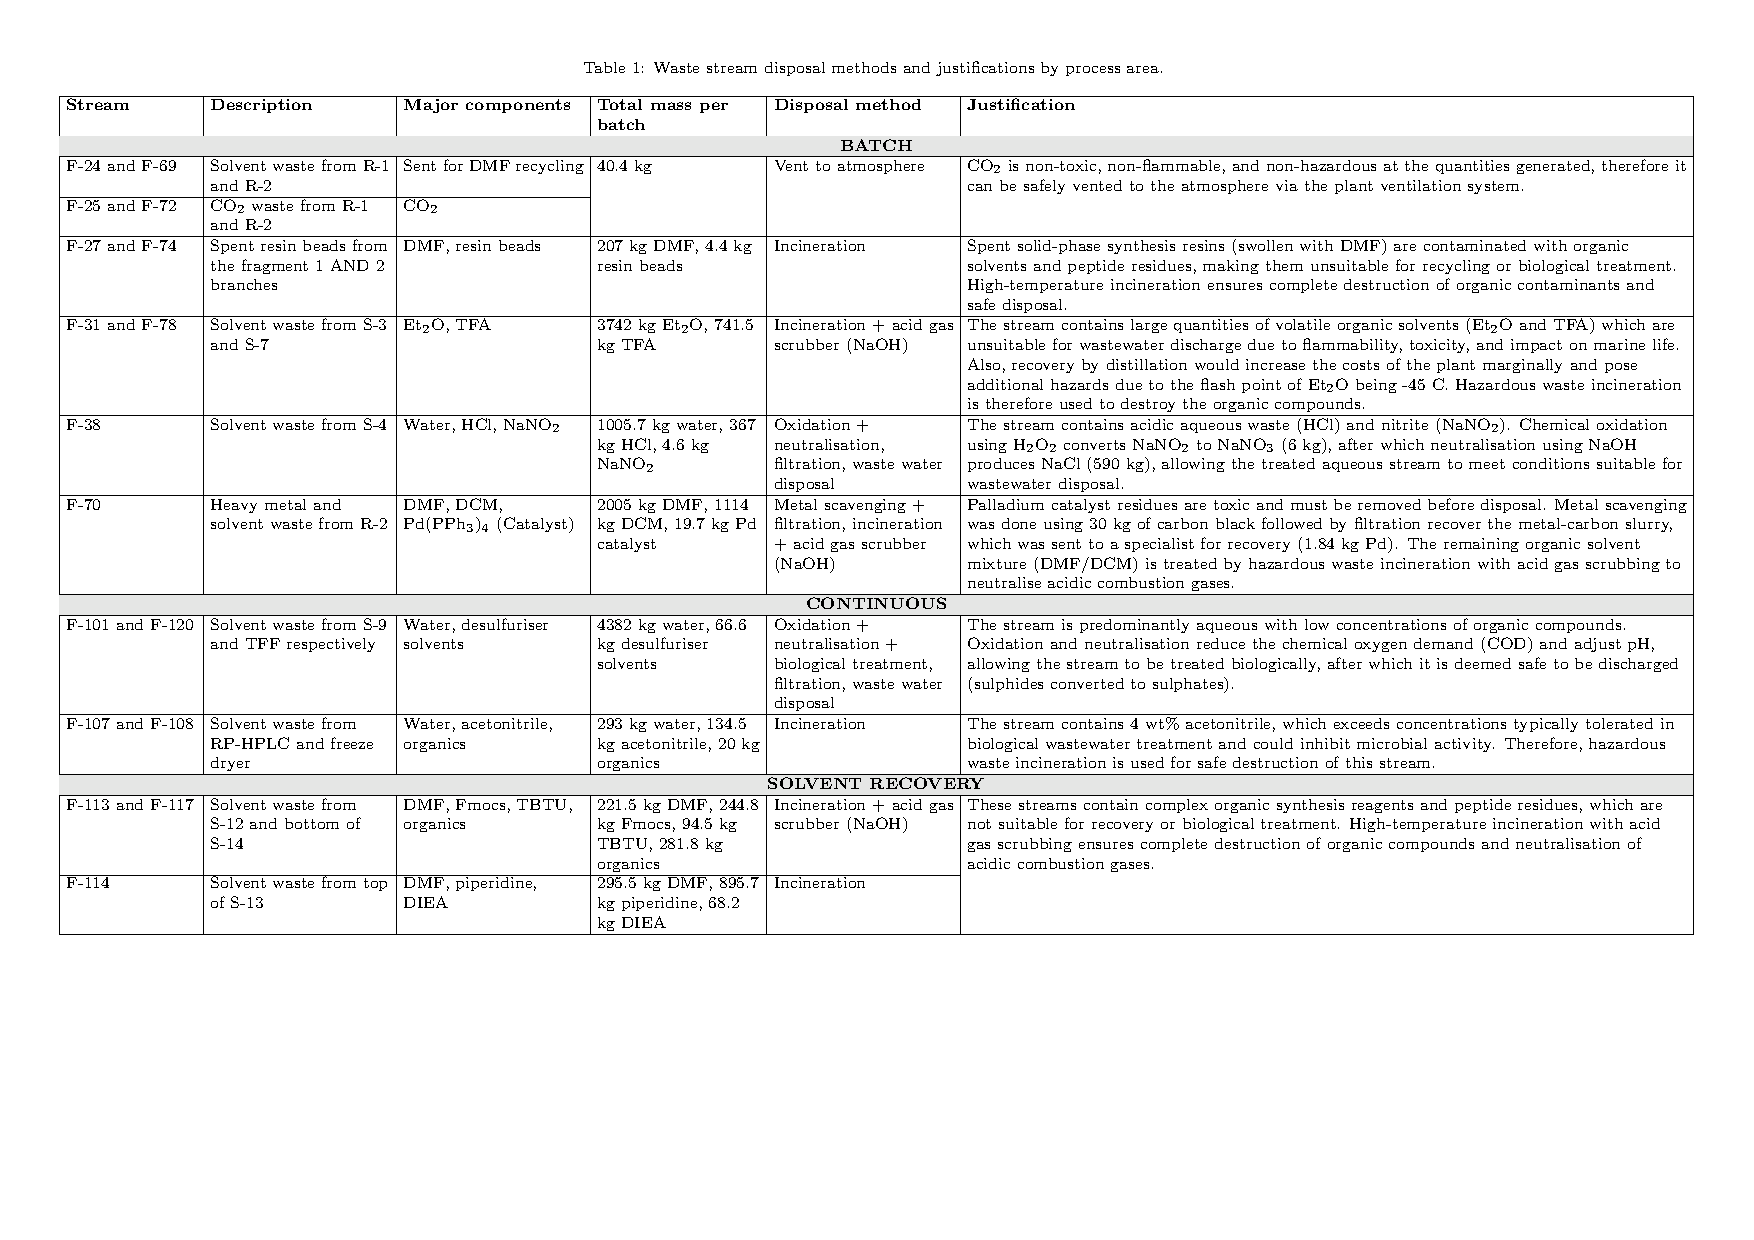
\includepdf[pages=-,landscape=true]{figures/tables/waste_stream_disposal_table.pdf}

Table~\ref{tab:emissions_effluents} summarises the main emissions and effluents generated from waste treatment and incineration, together with batch and annual quantities.

Appendix~\ref{app:incineration} shows the total mass of compounds sent for incineration as well as the corresponding NaOH requirement for flue gas scrubbing. Table~\ref{tab:emissions_effluents} shows the main emissions and effluents generated from the waste treatment and incineration processes, including their quantities.

\begin{table}[htbp]
    \centering
    \caption{Main emissions and effluents from waste treatment and incineration.}
    \label{tab:emissions_effluents}
    \small
    \begin{tabularx}{\textwidth}{|>{\raggedright\arraybackslash}X|c|c|>{\raggedright\arraybackslash}X|}
        \hline
        \textbf{Emissions/effluents} & \textbf{kg/batch} & \textbf{tons/year} & \textbf{Limits} \\
        \hline
        CO$_2$                       & 19600             & 1019.2             &                 \\
        \hline
        H$_2$O                       & 9220              & 479.44             &                 \\
        \hline
        NO$_x$                       & trace             & -                  &                 \\
        \hline
        HCl (removed in scrubber)    & 957               & 49.764             &                 \\
        \hline
        HF (removed in scrubber)     & 390               & 20.28              &                 \\
        \hline
        SO$_2$ (removed in scrubber) & 50                & 2.6                &                 \\
        \hline
        Waste water                  & 6250              & 325                &                 \\
        \hline
    \end{tabularx}
    \normalsize
\end{table}

Appendix~\ref{app:waste_treatment} summarises the chemicals and equipment required for the waste treatment plant, including chemical consumption per batch, equipment specifications, capital costs, and energy requirements. These data were used to estimate the annual cost of the waste treatment system, which was calculated to be \$342,085. The total waste generated by the process is approximately 19,240~kg per year, corresponding to a treatment cost of about \$0.34 per kg of waste.

It is to be noted that this estimate only includes capital costs for treatment equipment (e.g., incinerator, scrubber, oxidation and neutralisation tanks, filtration units, metal scavenging and biological treatment tanks) and operating costs for chemicals such as NaOH, carbon black, H\textsubscript{2}O\textsubscript{2}, biomass, and electricity. It does not include additional industrial costs such as labour, equipment maintenance, sludge disposal, emissions monitoring, regulatory compliance, or waste transport, which can significantly increase overall treatment costs in pharmaceutical facilities.

\subsection{Utilities}
\label{sec:utilities}

A detailed evaluation of the utilities required for plant operation is presented in this subsection. Excluding waste treatment, the total installed electrical load of the plant is 111.8~kW, corresponding to the combined power requirements of pumps and mixers. The plant also requires approximately 1~gpm of industrial water, equivalent to approximately 2000~m$^3$/year, which is subsequently purified using reverse osmosis and electrodeionisation for use in pharmaceutical processing. Additional utilities required to support process operation and temperature control include chilled water, propylene glycol-water brine refrigeration, and low- and medium-pressure steam, as described in this subsection.

From a sustainability perspective, the process incorporates solvent recovery and on-site waste treatment systems to reduce solvent consumption and minimise environmental emissions. In addition, propylene glycol-water brine was selected as the refrigeration medium rather than ethylene glycol due to its lower toxicity and favourable safety profile for pharmaceutical manufacturing.

\subsection{Greenhouse Gas Emissions}
\label{sec:ghg_emissions}

Carbon dioxide emissions from the plant include both direct (Scope~1) and indirect (Scope~2) sources. Annual Scope~1 CO$_2$ emissions are approximately 1,020~ton/year, primarily originating from process vents and incineration flue gases. Indirect CO$_2$ emissions (Scope~2) are estimated at approximately 600~ton/year, arising from the electricity demand of the main process and waste treatment operations, as well as the steam requirements of the plant. SO$_2$ and trace quantities of NO$_x$ are also produced during the incineration process, but these emissions are subsequently treated in a caustic scrubber, ensuring that they are not directly released to the environment. These values provide an overall estimate of the greenhouse gas emissions associated with the facility's operation. A summary of related emissions and treatment calculations is provided in Appendix~\ref{app:incineration} and Appendix~\ref{app:waste_treatment}.

The estimated emissions were compared with regulatory limits specified under the IED and the BAT conclusions for waste incineration and chemical sector emissions. Acid gases generated during incineration, including SO$_2$, HCl and HF, are removed through a caustic scrubbing system prior to atmospheric release. The predicted emission levels therefore remain below typical BAT-associated emission levels for these gases, demonstrating compliance with applicable environmental regulations.

Potential reductions in greenhouse gas emissions could be achieved through both operational and energy-sourcing strategies. Scope~1 emissions could be reduced by improving energy efficiency, recovering heat from incineration flue gases, or minimising the amount of waste sent for incineration through more efficient solvent recovery and waste reduction measures. Scope~2 emissions could be reduced by sourcing electricity from a lower-carbon energy mix than the current grid mix in North Carolina. This could include the use of renewable electricity through power purchase agreements or on-site renewable generation such as solar power. Increasing the proportion of renewable energy used to meet the plant's electricity demand would significantly reduce the indirect carbon footprint associated with process operation.


\input{chapters/4_conclusion}

\clearpage
\appendix

\section*{Appendix XX}
\addcontentsline{toc}{section}{Appendix XX}

\begin{table}[ht]
\centering
\caption{Likelihood classification used in the qualitative risk assessment.}
\label{tab:likelihood}
\begin{tabularx}{\textwidth}{|c|X|X|X|}
\hline
\textbf{} & \textbf{Likelihood} & \textbf{Probability} & \textbf{Frequency} \\
\hline
A & Improbable & $p_{\textit{once}} < 0.001$ & Less than once every 1000 years \\
\hline
B & Unlikely & $0.001 < p_{\textit{once}} < 0.01$ & Once every 100--1000 years \\
\hline
C & Possible & $0.01 < p_{\textit{once}} < 0.1$ & Once every 10--100 years \\
\hline
D & Probable & $0.1 < p_{\textit{once}} < 1$ & Once every 1--10 years \\
\hline
E & Frequent & $p_{\textit{several}} = 1$ & More than once a year \\
\hline
\end{tabularx}
\end{table}

\vspace{1em}

\begin{table}[ht]
\centering
\caption{Severity classification used in the qualitative risk assessment.}
\label{tab:severity}
\begin{tabularx}{\textwidth}{|c|X|X|X|X|}
\hline
\textbf{S} & \textbf{Severity} & \textbf{To people} & \textbf{To process plant} & \textbf{To environment} \\
\hline
I   & Minor        & First aid           & Barely any damage              & Negligible impact \\
\hline
II  & Moderate     & Medical care        & Repair needed                  & Short-term impact, minor contamination \\
\hline
III & Serious      & Disabling           & Loss of process unit           & Measurable, reversible impact \\
\hline
IV  & Very serious & One fatality        & Local destruction of the plant & Significant, long-term impact \\
\hline
V   & Severe       & Multiple fatalities & Complete destruction           & Permanent extreme impact \\
\hline
\end{tabularx}
\end{table}

\vspace{2em}

% Risk matrix
\newcolumntype{C}[1]{>{\centering\arraybackslash}m{#1}}
{\renewcommand{\arraystretch}{1.8}%
\begin{table}[ht]
\centering
\caption{Risk matrix: colour-coded by risk level (L = Low, M = Medium, H = High).}
\label{tab:riskmatrix}
\begin{tabular}{|C{2cm}|C{0.9cm}|C{2.4cm}|C{2.4cm}|C{2.4cm}|C{2.4cm}|C{2.4cm}|}
\hline
\cellcolor{riskGray}\multirow{5}{2cm}{\centering\textbf{Severity (S)}} &
  \cellcolor{riskDark}\textcolor{white}{V} &
  \cellcolor{riskM}\textcolor{white}{M} &
  \cellcolor{riskM}\textcolor{white}{M} &
  \cellcolor{riskH}\textcolor{white}{H} &
  \cellcolor{riskH}\textcolor{white}{H} &
  \cellcolor{riskH}\textcolor{white}{H} \\
\cline{2-7}
\cellcolor{riskGray} &
  \cellcolor{riskDark}\textcolor{white}{IV} &
  \cellcolor{riskM}\textcolor{white}{M} &
  \cellcolor{riskM}\textcolor{white}{M} &
  \cellcolor{riskH}\textcolor{white}{H} &
  \cellcolor{riskH}\textcolor{white}{H} &
  \cellcolor{riskH}\textcolor{white}{H} \\
\cline{2-7}
\cellcolor{riskGray} &
  \cellcolor{riskDark}\textcolor{white}{III} &
  \cellcolor{riskM}\textcolor{white}{M} &
  \cellcolor{riskM}\textcolor{white}{M} &
  \cellcolor{riskM}\textcolor{white}{M} &
  \cellcolor{riskH}\textcolor{white}{H} &
  \cellcolor{riskH}\textcolor{white}{H} \\
\cline{2-7}
\cellcolor{riskGray} &
  \cellcolor{riskDark}\textcolor{white}{II} &
  \cellcolor{riskL}\textcolor{white}{L} &
  \cellcolor{riskL}\textcolor{white}{L} &
  \cellcolor{riskM}\textcolor{white}{M} &
  \cellcolor{riskM}\textcolor{white}{M} &
  \cellcolor{riskH}\textcolor{white}{H} \\
\cline{2-7}
\cellcolor{riskGray} &
  \cellcolor{riskDark}\textcolor{white}{I} &
  \cellcolor{riskL}\textcolor{white}{L} &
  \cellcolor{riskL}\textcolor{white}{L} &
  \cellcolor{riskL}\textcolor{white}{L} &
  \cellcolor{riskL}\textcolor{white}{L} &
  \cellcolor{riskM}\textcolor{white}{M} \\
\hline
\multicolumn{2}{|c|}{} &
  \cellcolor{riskDark}\textcolor{white}{A} &
  \cellcolor{riskDark}\textcolor{white}{B} &
  \cellcolor{riskDark}\textcolor{white}{C} &
  \cellcolor{riskDark}\textcolor{white}{D} &
  \cellcolor{riskDark}\textcolor{white}{E} \\
\hline
\multicolumn{2}{|c|}{} &
  \multicolumn{5}{c|}{\cellcolor{riskDark}\textcolor{white}{\textbf{Likelihood (L)}}} \\
\hline
\end{tabular}
\end{table}}

\clearpage
\subsection*{Appendix: Incineration Calculations}
\label{app:incineration}

\begin{table}[htbp]
\centering
\caption{Compounds sent to incineration and NaOH requirement for scrubbing.}
\label{tab:incineration_summary}
\small
\begin{tabularx}{\textwidth}{|>{\raggedright\arraybackslash}X|c|c|c|c|}
\hline
\textbf{Compound} & \textbf{kg/batch} & \textbf{kg/year} & \textbf{kg/hour} & \textbf{NaOH scrubbing (kg/batch)} \\
\hline
DMF & 2729 & 141908 & 17.7385 & 0 \\
\hline
resin & 4.4 & 228.8 & 0.0286 & 0 \\
\hline
Et$_2$O & 3742 & 194584 & 24.323 & 0 \\
\hline
TFA & 741.5 & 38558 & 4.81975 & 260 \\
\hline
DCM & 1114 & 57928 & 7.241 & 1050 \\
\hline
ACN & 134.5 & 6994 & 0.87425 & 0 \\
\hline
Fmocs & 244.8 & 12729.6 & 1.5912 & 0 \\
\hline
TBTU & 94.5 & 4914 & 0.61425 & 0 \\
\hline
Organics & 281.8 & 14653.6 & 1.8317 & 0 \\
\hline
Piperidine & 895.7 & 46576.4 & 5.82205 & 0 \\
\hline
DIEA & 68.2 & 3546.4 & 0.4433 & 0 \\
\hline
Others (25 kg halide/S compounds) & 200 & 10400 & 1.3 & 30 \\
\hline
Total & 10250.4 & 533020.8 & 66.6276 & 1340 \\
\hline
\end{tabularx}
\normalsize
\end{table}

\clearpage
\subsection*{Appendix: Waste Treatment Requirements}
\label{app:waste_treatment}

\begin{table}[htbp]
\centering
\caption{Waste treatment chemicals and annual costs.}
\label{tab:waste_treatment_chemicals}
\small
\begin{tabularx}{\textwidth}{|>{\raggedright\arraybackslash}X|c|c|>{\raggedright\arraybackslash}X|}
\hline
\textbf{Chemicals total} & \textbf{kg/batch} & \textbf{Annual cost (\$)} & \textbf{Purpose} \\
\hline
NaOH & 2500 & 97500 & Scrub + neutralisation \\
\hline
Carbon black & 30 & 1996.8 & Pd scavenging \\
\hline
H$_2$O$_2$ 30\% solution & 25 & 1196 & Oxidation \\
\hline
Activated biomass & 60 & 64428 & Biological treatment (85 kg organics) \\
\hline
Total &  & 165120.8 & \\
\hline
\end{tabularx}
\normalsize
\end{table}

\begin{table}[htbp]
\centering
\caption{Waste treatment equipment, sizing, and annual energy demand.}
\label{tab:waste_treatment_equipment}
\small
\begin{tabularx}{\textwidth}{|>{\raggedright\arraybackslash}X|c|>{\raggedright\arraybackslash}X|c|c|}
\hline
\textbf{Equipment} & \textbf{Units} & \textbf{Size} & \textbf{Cost} & \textbf{Energy required (kWh/yr)} \\
\hline
Incinerator & 1 & 1.3 x 2.4 x 8.1m & 35000 & 800000 \\
\hline
Scrubber & 1 & 4 x 1.5 x 4m & 2500 & 10800 \\
\hline
Oxidation tank & 1 & 100L & 5355 & 10800 \\
\hline
Neutralisation tank & 1 & 100L & 5355 & 10800 \\
\hline
Filter & 2 & 1.2 x 0.6 x 0.6m & 300 & 10800 \\
\hline
Metal scavenging tank & 1 & 100L & 5355 & 10800 \\
\hline
Biological treatment tank & 1 & 100L & 2000 & 11000 \\
\hline
Total &  &  & 55865 & 865000 \\
\hline
\end{tabularx}
\normalsize
\end{table}


\clearpage
\printbibliography

\end{document}
